
\documentclass[article]{IEEEtran}
\usepackage{graphicx}
 \usepackage{url}
\usepackage{amsmath}
\setlength{\parskip}{0.5em}
\setlength{\parindent}{2em}

\begin{document}

\title{Fundamentals of Artificial Intelligence Assignment 2- Solving the Travelling Salesman Problem with Genetic Algorithms}

\author{\IEEEauthorblockN{Craig Heptinstall}
\IEEEauthorblockA{Crh13- 110005643\\SEM6120\\
Institute of Computer Science\\
Aberystywth University}}

\maketitle

\begin{abstract}
Genetic algorithms provide an optimization technique for a wide variety of problems, including that of the travelling salesman. The number of solutions for a TSP can become exponential, which genetic algorithms such as roulette, tournament and others can help reduce the number of evaluated solutions vastly. 
\end{abstract}

\section{Introduction}
Genetic algorithms are considered in a wide array of problems where exact algorithms would struggle. The travelling salesman problem is a great example of a problem that does not have a means of finding the best solution first time, and would be increasingly time consuming to loop through all possible solutions to find the lowest cost (length of path).

\subsection{Travelling Salesman Problem}
To understand the travelling salesman problem, the reasons for its existence and early sources should be known. The travelling salesman problem was thought up in 1930 \cite{1} by Merrill Flood whilst looking to solve a school bus routing problem. The problem stems off from the Hamiltonian cycle puzzle, requiring the solver to visit all node or ‘cities’ once in a set of \( \mathcal{N} \) cities. At this point in time, no general method of solution is known \cite{2} (so is considered NP-hard) therefore only the best and shortest paths can be evaluated from several attempts. \par
Because of the nature of the problem, genetic algorithms appear as an idealistic means of finding optimised tours where a solution cannot be found using a mathematical means. Evolutionary algorithms used in genetics may never be guaranteed to find optimal solutions, though due to their random nature they will often find a good solution \cite{3}. Genetic algorithms are called as so because of the similar way they act to natural selection, with the best and most efficient parents creating more advantageous children. In the instance of the travelling salesman, this could be reflected where two parents whose path distances are short are combined to form a child who uses similar paths to that of its parents, combined with a small form of randomness in the hope of improving upon a solution. \par
Figures \ref{fig:1} and \ref{fig:2} show an example TSP with a low number of points where an optimal solution can be found quite easily by exact, heuristic or GA means. An important aspect expressed in figure 2 is that although all the points are visited, the final vertex visited must also be linked to the first in order to return to the starting position.
\begin{figure}
\centering
  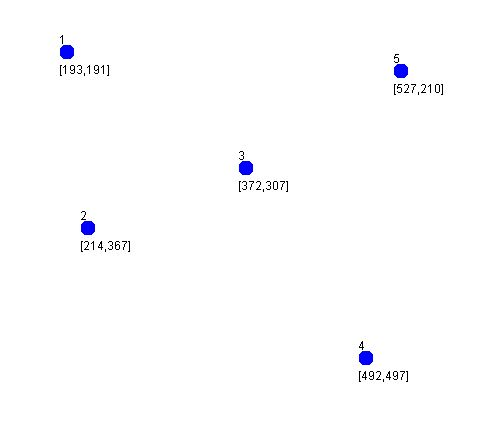
\includegraphics[width=.8\linewidth]{images/problem}
  \caption{An example set of vertices where a travelling salesman problem is present.}
  \label{fig:1}
\end{figure}
\begin{figure}
\centering
  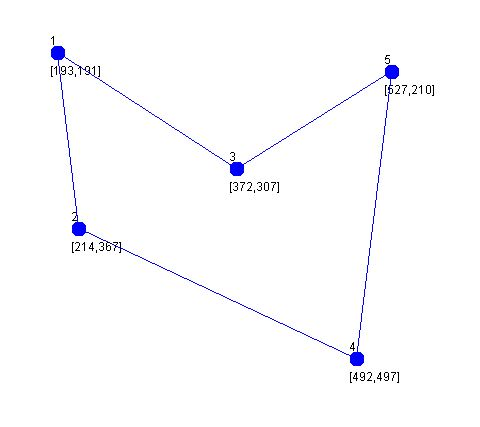
\includegraphics[width=.8\linewidth]{images/solution}
  \caption{A possible solution to the TSP expressed above.}
  \label{fig:2}
\end{figure}

\section{Genetic algorithms considered for TSP}
Before looking at the possible genetic algorithms to be considered for such a puzzle as the TSP, it should be understood that a very basic generic algorithm can be used for such a purpose. In a paper in the Scientific World Journal \cite{4}, a team worked on using a traditional algorithm created back in 1989 by David Goldberg \cite{5} and improving its efficiency to help solve the TSP quickly and as accurately as possible. The original genetic algorithm, which many algorithms are based from today goes through the following process:
\begin{enumerate}
\item Randomly generate an initial population of chromosomes.
\item Use the fitness function to select the fitter chromosomes.
\item Apply the crossover and mutation operators in order. 
\item If a stopping criterion is satisfied, then stop and output the best chromosome
\item Go to step 2
\end{enumerate}

\section{Proposed solution}

\subsection{Selected and considered GA's}

\subsection{Application structure}

\subsection{Comparison of application results}

\section{Overall findings and conclusion}

\subsection{Improvements to proposed solution}

\begin{thebibliography}{9}

\bibitem{1} 
E.L. Lawler, \textit{The Traveling salesman problem : a guided tour of combinatorial optimization},
1985

\bibitem{2} 
E.W. Weisstein, \textit{Hamiltonian Cycle},
\textit{\url{http://mathworld.wolfram.com/HamiltonianCycle.html}}, 2015

\bibitem{3} 
D.W. Dyer, \textit{When are Evolutionary Algorithms Useful?},
\textit{\url{http://watchmaker.uncommons.org/manual/ch01s02.html}}, 2008

\bibitem{4} 
C.W. Tsai, S.P Tseng, M.C. Chiang, C.S. Yang, T.P. Hong, \textit{A High-Performance Genetic Algorithm: Using Traveling Salesman Problem as a Case},
The Scientific World Journal Volume 2014, 2014

\bibitem{5}
D.E. Goldberg, \textit{Genetic Algorithms in Search, Optimization, and Machine Learning},
Addison-Wesley Longman Publishing Co., 1989. 

\end{thebibliography}
\end{document}


